\section{Jet flavour tagging}
\label{sec:ch6_btag}

Jet flavour tagging is used to distinguish jets originating from $b$-quarks ($b$-jets) from other jet flavours.

$b$-jets are identified through the displaced decays of $b$-hadrons, which have a lifetime of about $1.5~\ps$. A boosted $b$-hadron can therefore travel several millimetres before decaying.
The decay tracks therefore typically have large impact parameters and originate from a secondary vertex displaced from the PV.
Charm hadrons produced in the $b$-hadron decay can further decay at an additional displaced vertex.
These features are used for jet flavour tagging.

The tagger uses the GN2v01 algorithm, which is based on a transformer neural network trained on simulated events~\cite{ATLAS2026GN2}.
Its inputs include jet and track kinematics, impact parameters, and hit variables.
The network is illustrated in Figure~\ref{fig:ch6_gn2}. It consists of a transformer network and a jet-flavour classifier.

The jet-flavour classifier outputs the discriminant for the jet flavour classification. The larger values of the discriminant favour the $b$-jet hypothesis.
The GN2v01 85\% working point is used in this analysis, corresponding to a nominal $b$-jet tagging efficiency of 85\%.
The representative rejection rates against light-jets and $c$-jets are about 98.6\% and 83\%, respectively.

% These variables are first encoded as a numerical vector for each track.
% Within the transformer, each vector is updated through self-attention, using information from the other tracks.
% Correlations between tracks can thereby be used to recognise a common displaced origin without requiring explicitly reconstructed secondary vertices as separate inputs.
% The network then calculates a weight for each track using its updated vector and adds the weighted vectors together, which is called attention pooling.

% The resulting vector is used for the main task of jet-flavour classification.
% It is also combined with the individual track vectors for two auxiliary tasks: identifying track origins and predicting whether pairs of tracks originate from the same vertex.
% The three tasks share the transformer and are trained jointly, helping it learn the decay structure.
% The network and its three tasks are is illustrated in Figure~\ref{fig:ch6_gn2}.

% The jet-flavour classifier produces four outputs for the $b$-jet, $c$-jet, hadronic-$\tau$ and light-jet hypotheses, where light jets originate from $u$, $d$ or $s$ quarks or gluons.
% These outputs are combined into a single discriminant, $D_b$, which compares the $b$-jet output with a weighted combination of the other three outputs.
% Larger values favour the $b$-jet hypothesis.
% The GN2v01 85\% working point is used in this analysis, corresponding to a nominal $b$-jet tagging efficiency of 85\%.

\begin{figure}[htbp]
    \centering
    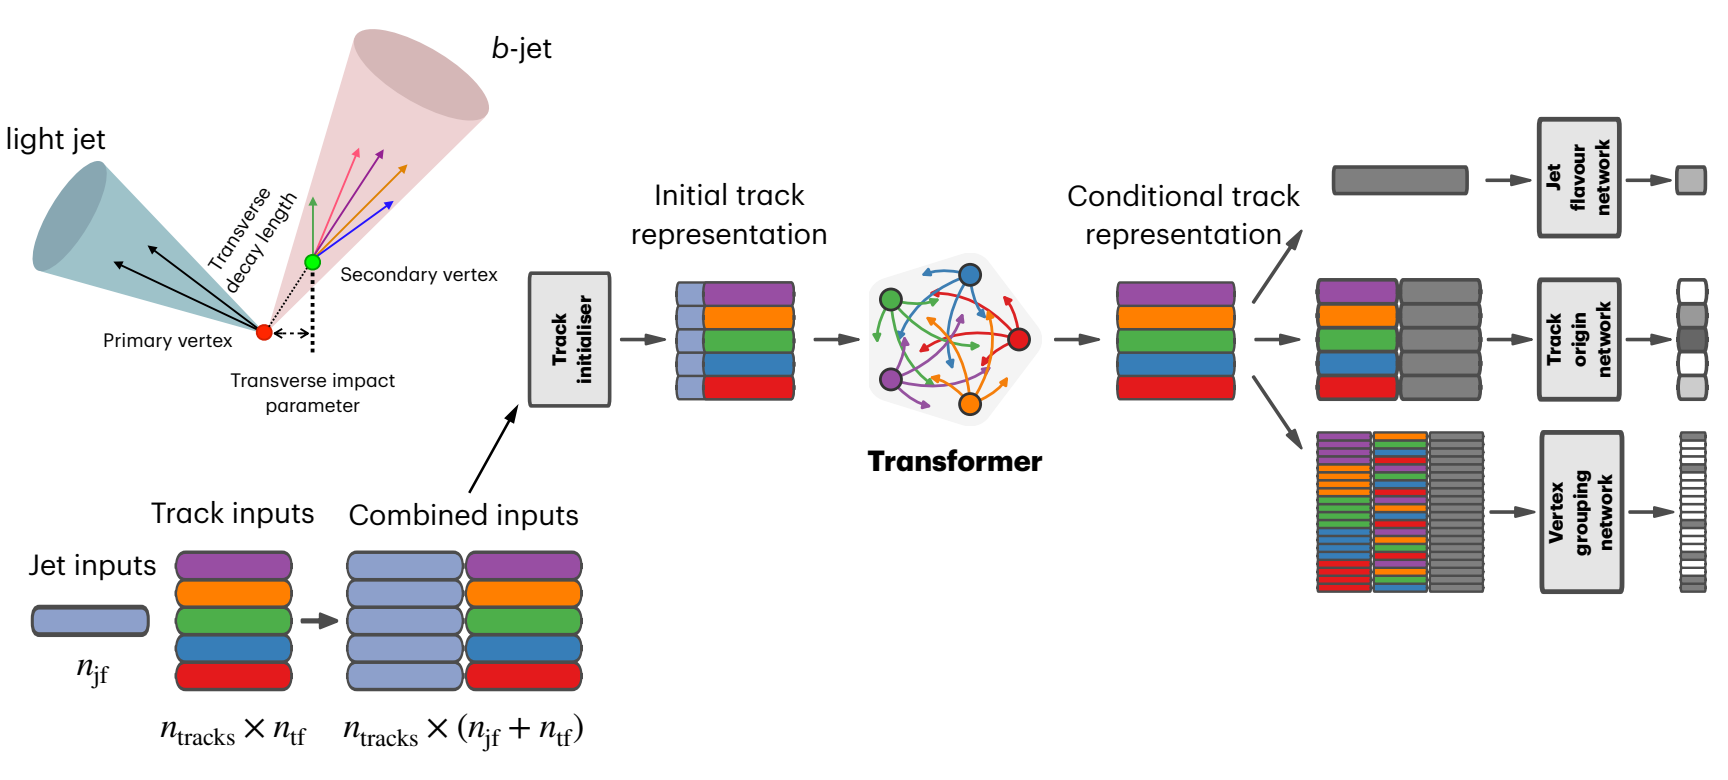
\includegraphics[width=\textwidth]{Figs/CH6/gn2_architecture.png}
    \caption[GN2 flavour-tagging architecture]{GN2 flavour-tagging architecture. The jet variables are appended to the input vector of each track before processing by the track initialiser and transformer. The resulting track vectors and their weighted combination are passed to the jet-flavour, track-origin and vertex-grouping networks. The symbols $n_{\mathrm{jf}}$, $n_{\mathrm{tf}}$ and $n_{\mathrm{tracks}}$ denote the numbers of jet variables, track variables and tracks, respectively~\cite{ATLAS2026GN2}.}
    \label{fig:ch6_gn2}
\end{figure}

\subsection{Calibration}

The $b$-jet tagging efficiency is measured in dileptonic $\ttbar$ events with an opposite-charge electron--muon pair and two jets.
The $c$-jet mistagging efficiency, the probability for a $c$-jet to pass the $b$-tagging requirement, is measured in semileptonic $\ttbar$ events using charm jets from hadronic $W$ decays.
The corresponding light-jet mistagging efficiency is measured in $Z$+jets events with $\zee$ or $\zmumu$ decays~\cite{ATLAS2026GN2}.

These efficiencies are measured in jet $\pT$ bins and compared with simulation to obtain scale factors that depend on the true jet flavour, as defined in Eq.~\eqref{eq:ch6_efficiency_sf}.
Corrections are then applied to the simulated event weights for both jets that pass the discriminator threshold (tagged jets) and those that fail it (untagged jets).
The light-jet and $c$-jet rejections before and after calibration are shown as functions of the $b$-jet tagging efficiency in Figure~\ref{fig:ch6_btag_calibration}.

\begin{figure}[htpb]
    \centering
    \begin{subfigure}{0.49\textwidth}
        \centering
        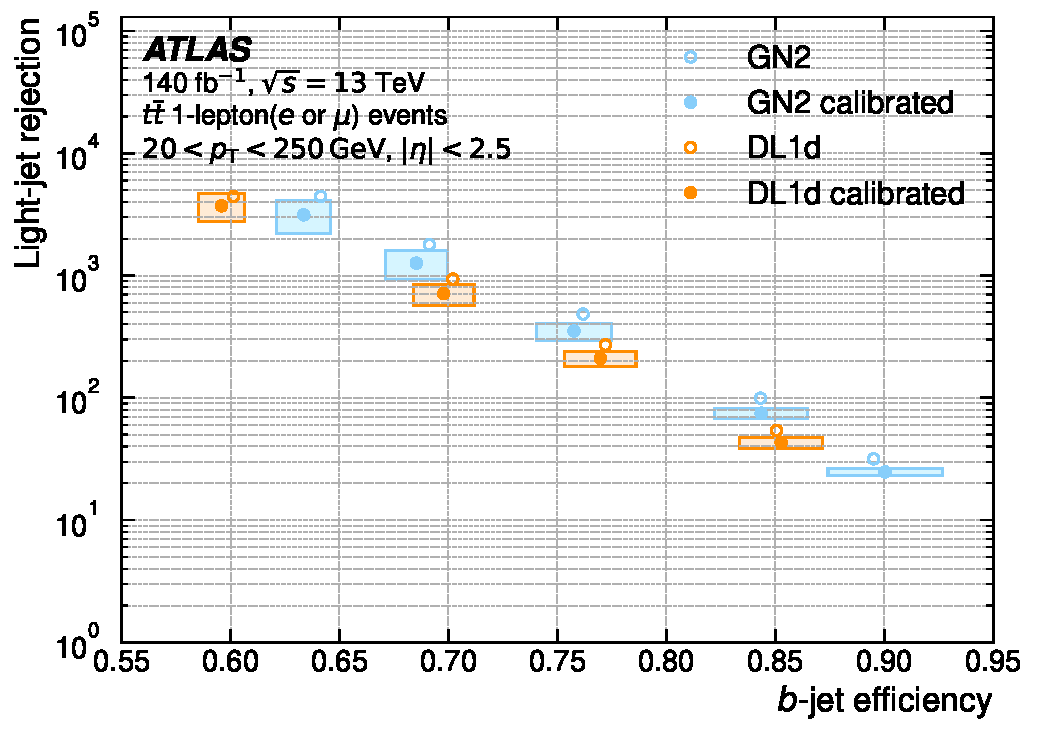
\includegraphics[width=\linewidth]{Figs/CH6/gn2_light_rejection.pdf}
        \caption{Light-jet rejection.}
    \end{subfigure}
    \hfill
    \begin{subfigure}{0.49\textwidth}
        \centering
        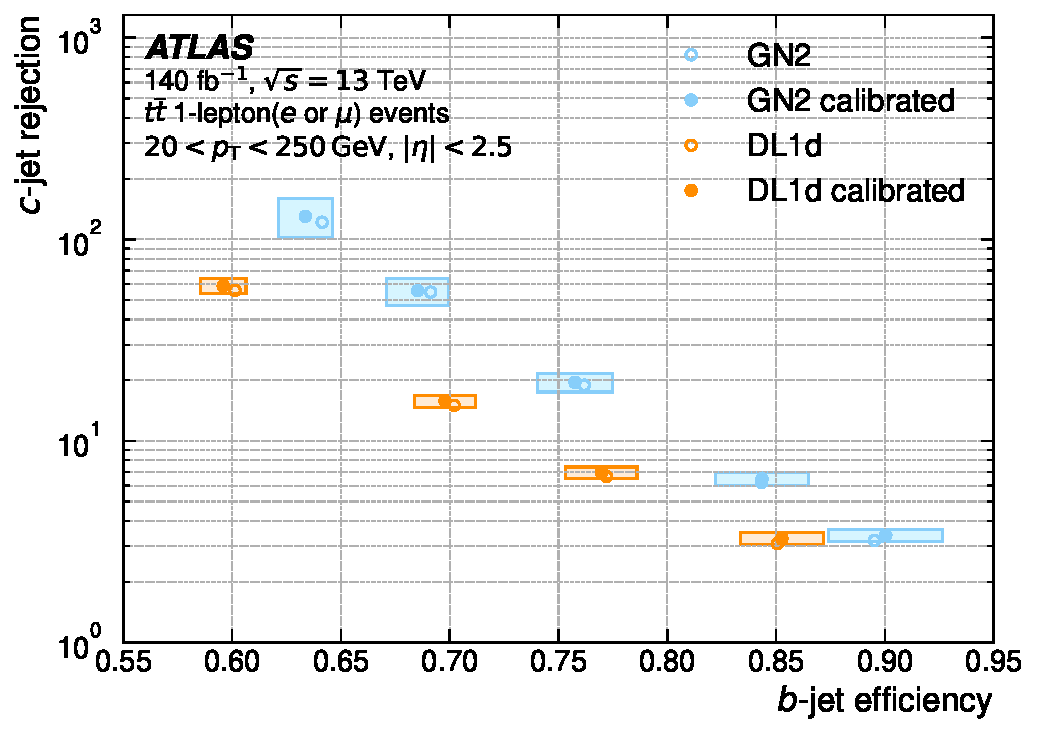
\includegraphics[width=\linewidth]{Figs/CH6/gn2_c_rejection.pdf}
        \caption{$c$-jet rejection.}
    \end{subfigure}
    \caption[GN2 flavour-tagging performance]{Light-jet (a) and $c$-jet (b) rejection as functions of the $b$-jet tagging efficiency for GN2 (blue) and DL1d (orange) in $\ttbar$ events~\cite{ATLAS2026GN2}. Rejection is defined as the inverse mistagging efficiency. Open circles show the simulation predictions, and filled circles show the results measured in Run~2 data. The horizontal and vertical bands show the uncertainties in the $b$-jet efficiency and background rejection, respectively.}
    \label{fig:ch6_btag_calibration}
\end{figure}
